\documentclass[twocolumn]{article}
\usepackage{amsmath}
\usepackage{xcolor-material}
\usepackage{pgfplots}
\usepackage{float}
\usepackage{caption}
\usepackage{graphicx}
\usepackage{amssymb}
\usepackage{geometry}
\usepackage{diagbox}
\usepackage{float}
\usepackage{enumitem}
\usepackage{array}
\usepackage{booktabs}
\usepackage{tabularray}
\usepackage{makecell}
\usepackage{csquotes}
\usepackage{tikz}
\usepackage[ruled,linesnumbered]{algorithm2e}
\usetikzlibrary{positioning,arrows.meta}
\usepackage{upgreek}
\usepackage{titling}
\geometry{a4paper, left=0.5in, right=0.5in, top=0.5in, bottom=0.7in}
\usepackage[skip=6pt]{parskip}
\setlength{\droptitle}{-0.35in}
\captionsetup{belowskip=0pt}

\setitemize{noitemsep,topsep=2pt,parsep=6pt,}
\setlength{\parindent}{0pt}

\captionsetup{justification=centering}

\let\oldnl\nl
\newcommand{\nonl}{\renewcommand{\nl}{\let\nl\oldnl}}

\title{IPCV Cheatsheet}
\author{ArneshRC}
\date{}

\begin{document}

\maketitle

\section*{Introduction}

\subsection*{Digital Images}

A \textbf{digital image} is a representation of a two-dimensional
image as a finite $M \times N$ matrix of digital values, called
picture elements or \textbf{pixels}.

\begin{itemize}
  \item Pixel values typically represent gray levels (often 0 - 255),
    colours, heights, opacities etc.
  \item \textit{Digitization} implies that a digital image is an
    \textbf{approximation} of a real scene.
  \item Common image formats: (i) one sample per point (B \& W,
    Grayscale), (ii) three samples per point (RGB), (iii) four
    samples per point (RGBA).
\end{itemize}

\subsection*{Digital Image Processing}

Two major tasks:

\begin{itemize}
  \item Improvement of pictorial information for human
    interpretation. Examples: image enhancement, image restoration.
  \item Proessing of image data for storage, transmission and
    representation for autonomous machine perception. Examples: image
    segmentation, object recognition, image classification.
\end{itemize}

\subsubsection*{Image Processing $\rightarrow$ Computer Vision Continuum:}

\noindent
%─── First box ───
\begin{minipage}[t]{0.3\linewidth}
  \begin{tblr}{
      width   = \linewidth,
      colspec = { X[c] },
      row{1}  = { font=\bfseries },
      hlines, vlines
    }
    Low-Level Process \\
    \parbox[c][12em][b]{\linewidth}{%
      \textbf{Input}:\\ Image\\
      \textbf{Output}:\\ Image
      \vfill
      \textbf{Examples}: Noise removal, image sharpening
    }
  \end{tblr}
\end{minipage}\hfill
\begin{minipage}[t]{0.3\linewidth}
  \begin{tblr}{
      width   = \linewidth,
      colspec = { X[c] },
      row{1}  = { font=\bfseries },
      hlines, vlines
    }
    Mid-Level Process \\
    \parbox[c][12em][b]{\linewidth}{%
      \textbf{Input}:\\ Image\\
      \textbf{Output}:\\ Attributes
      \vfill
      \textbf{Examples}: Object recognition, image segmentation
    }
  \end{tblr}
\end{minipage}\hfill
\begin{minipage}[t]{0.3\linewidth}
  \begin{tblr}{
      width   = \linewidth,
      colspec = { X[c] },
      row{1}  = { font=\bfseries },
      hlines, vlines
    }
    High-Level Process \\
    \parbox[c][12em][b]{\linewidth}{%
      \textbf{Input}:\\ Attributes\\
      \textbf{Output}:\\ Understanding
      \vfill
      \textbf{Examples}: Scene understanding, autonomous navigation
    }
  \end{tblr}
\end{minipage}

\subsubsection*{Key Stages in Digital Image Processing:}

\begin{figure}[H]
  \centering
  \begin{tikzpicture}[
      node distance=0.8cm and 0.6cm,
      every node/.style={
        draw,
        rectangle,
        minimum width=2.61cm,
        text width=2.3cm,
        align=center
      },
      >={Stealth} % arrow tip
    ]
    % Row 1
    \node (n1) {Image Acquisition};
    \node (n2) [right=of n1] {Image Enhancement};
    \node (n3) [right=of n2] {Image Restoration};

    % Row 2
    \node (n4) [below=of n3] {Morphological Processing};
    \node (n5) [left=of n4] {Segmentation};
    \node (n6) [left=of n5] {Object Recognition};

    % Row 3
    \node (n7) [below=of n6] {Representation \& Description};
    \node (n8) [right=of n7] {Image Compression};
    \node (n9) [right=of n8] {Color Image Processing};

    % Sequential arrows
    \draw[->] (n1) -- (n2);
    \draw[->] (n2) -- (n3);
    \draw[->] (n3) -- (n4);
    \draw[->] (n4) -- (n5);
    \draw[->] (n5) -- (n6);
    \draw[->] (n6) -- (n7);
    \draw[->] (n7) -- (n8);
    \draw[->] (n8) -- (n9);
  \end{tikzpicture}
\end{figure}

\subsection*{Formation of Digital Images}

\begin{enumerate}
  \item \textbf{Image Acquisition:} Illuminate a scene, absorb the
    energy reflected by objects in the scene (various examples: (i)
      x-rays of skeletons, (ii) ultrasounds of unborn babies, (iii)
    electro-microscopic images of molecules).
  \item \textbf{Image Sensing:} Energy lands on sensor material
    responsive to that type of energy, generates a voltage.
    Collections of sensors are \textbf{arranged} to capture images.
  \item \textbf{Image Sampling:} Continuous image $\rightarrow$
    finite set of values (\enquote{grid of pixels}). Finer sampling
    $\rightarrow$ more pixels, more detail. \textbf{Determines
    spatial resolution}.
  \item \textbf{Image Quantization:} For each pixel, continuous value
    $\rightarrow$ value from finite set (e.g. whole number in 0 -
    255). \textbf{Determines intensity level resolution}.
\end{enumerate}

\subsection*{Relationships between Pixels}

\subsubsection*{Neighborhood}

For a pixel $p$ at position $(x, y)$:

\begin{itemize}
  \item \textbf{$N_4$:} $(x + 1, y), (x - 1, y), (x, y + 1), (x, y - 1)$.
  \item \textbf{$N_D$:} $(x + 1, y + 1), (x - 1, y + 1), (x + 1, y -
    1), (x - 1, y - 1)$.
  \item \textbf{$N_8$:} $N_4 \cup N_D$.

\end{itemize}

\noindent
\begin{minipage}{0.3\linewidth}
  \begin{tblr}{
      hlines, vlines,
      colspec={c},
      row{1}={font=\bfseries, c, m}
    }
    4-neighbors \\
    \begin{tikzpicture}[scale=0.6]
      \draw[step=1,gray,very thin] (-1.5,-1.5) grid (2.5,2.5);
      \fill[MaterialBlue200] (0,0)   rectangle (1,1);
      \fill[MaterialRed100]  (1,0)   rectangle (2,1);
      \fill[MaterialRed100]  (-1,0)  rectangle (0,1);
      \fill[MaterialRed100]  (0,1)   rectangle (1,2);
      \fill[MaterialRed100]  (0,-1)  rectangle (1,0);
    \end{tikzpicture}
  \end{tblr}
\end{minipage}\hfill
\begin{minipage}{0.3\linewidth}
  \begin{tblr}{
      hlines, vlines,
      colspec={c},
      row{1}={font=\bfseries, c, m}
    }
    D-neighbors \\
    \begin{tikzpicture}[scale=0.6]
      \draw[step=1,gray,very thin] (-1.5,-1.5) grid (2.5,2.5);
      \fill[MaterialBlue200] (0,0)   rectangle (1,1);
      \fill[MaterialRed100]  (1,1)   rectangle (2,2);
      \fill[MaterialRed100]  (-1,1)  rectangle (0,2);
      \fill[MaterialRed100]  (1,-1)  rectangle (2,0);
      \fill[MaterialRed100]  (-1,-1) rectangle (0,0);
    \end{tikzpicture}
  \end{tblr}
\end{minipage}\hfill
\begin{minipage}{0.3\linewidth}
  \begin{tblr}{
      hlines, vlines,
      colspec={c},
      row{1}={font=\bfseries, c, m}
    }
    8-neighbors \\
    \begin{tikzpicture}[scale=0.6]
      \draw[step=1,gray,very thin] (-1.5,-1.5) grid (2.5,2.5);
      \fill[MaterialBlue200] (0,0)   rectangle (1,1);
      \fill[MaterialRed100]  (1,0)   rectangle (2,1);
      \fill[MaterialRed100]  (-1,0)  rectangle (0,1);
      \fill[MaterialRed100]  (0,1)   rectangle (1,2);
      \fill[MaterialRed100]  (0,-1)  rectangle (1,0);
      \fill[MaterialRed100]  (1,1)   rectangle (2,2);
      \fill[MaterialRed100]  (-1,1)  rectangle (0,2);
      \fill[MaterialRed100]  (1,-1)  rectangle (2,0);
      \fill[MaterialRed100]  (-1,-1) rectangle (0,0);
    \end{tikzpicture}
  \end{tblr}
\end{minipage}

\subsubsection*{Adjacency}

For two pixels $p$ and $q$:
\begin{itemize}
  \item \textbf{4-adjacency:} $q \in N_4(p)$
  \item \textbf{8-adjacency:} $q \in N_8(p)$
  \item \textbf{m-adjacency:} (i) $q \in N_4(p)$ \textbf{or} (ii) $q
    \in N_D(p)$ and $N_4(p) \cap N_4(q) \nsubseteq \mathbf{V}$
\end{itemize}

\noindent
\begin{minipage}{0.3\linewidth}
  \begin{tblr}{
      hlines, vlines,
      colspec={c},
      row{1}={font=\bfseries, c, m}
    }
    4-adjacency \\
    \begin{tikzpicture}[scale=0.6]
      % grid and pixel array
      \draw[step=1,gray,very thin] (-0.5,-0.5) grid (3.5,3.5);
      \fill[MaterialBlue200] (1,2) rectangle ++(1,1);
      \fill[MaterialBlue200] (2,2) rectangle ++(1,1);
      \fill[MaterialBlue200] (1,1) rectangle ++(1,1);
      \fill[MaterialBlue200] (2,0) rectangle ++(1,1);
      % 4-adjacency connections
      \draw[MaterialRed600,dashed,very thick] (1.5,2.5) -- (2.5,2.5);
      \draw[MaterialRed600,dashed,very thick] (1.5,2.5) -- (1.5,1.5);
    \end{tikzpicture}
  \end{tblr}
\end{minipage}\hfill
\begin{minipage}{0.3\linewidth}
  \begin{tblr}{
      hlines, vlines,
      colspec={c},
      row{1}={font=\bfseries, c, m}
    }
    8-adjacency \\
    \begin{tikzpicture}[scale=0.6]
      % grid and pixel array
      \draw[step=1,gray,very thin] (-0.5,-0.5) grid (3.5,3.5);
      \fill[MaterialBlue200] (1,2) rectangle ++(1,1);
      \fill[MaterialBlue200] (2,2) rectangle ++(1,1);
      \fill[MaterialBlue200] (1,1) rectangle ++(1,1);
      \fill[MaterialBlue200] (2,0) rectangle ++(1,1);
      % 8-adjacency connections
      \draw[MaterialRed600,dashed,very thick] (1.5,2.5) -- (2.5,2.5);
      \draw[MaterialRed600,dashed,very thick] (1.5,2.5) -- (1.5,1.5);
      \draw[MaterialRed600,dashed,very thick] (1.5,1.5) -- (2.5,2.5);
      \draw[MaterialRed600,dashed,very thick] (1.5,1.5) -- (2.5,0.5);
    \end{tikzpicture}
  \end{tblr}
\end{minipage}\hfill
\begin{minipage}{0.3\linewidth}
  \begin{tblr}{
      hlines, vlines,
      colspec={c},
      row{1}={font=\bfseries, c, m}
    }
    m-adjacency \\
    \begin{tikzpicture}[scale=0.6]
      % grid and pixel array
      \draw[step=1,gray,very thin] (-0.5,-0.5) grid (3.5,3.5);
      \fill[MaterialBlue200] (1,2) rectangle ++(1,1);
      \fill[MaterialBlue200] (2,2) rectangle ++(1,1);
      \fill[MaterialBlue200] (1,1) rectangle ++(1,1);
      \fill[MaterialBlue200] (2,0) rectangle ++(1,1);
      % 4-adjacency connections
      \draw[MaterialRed600,dashed,very thick] (1.5,2.5) -- (2.5,2.5);
      \draw[MaterialRed600,dashed,very thick] (1.5,2.5) -- (1.5,1.5);
      % m-adjacency diagonal (only center to bottom-right)
      \draw[MaterialRed600,dashed,very thick] (1.5,1.5) -- (2.5,0.5);
    \end{tikzpicture}
  \end{tblr}
\end{minipage}

\subsubsection*{Connectivity}

\begin{itemize}
  \item Pixels $p, q$ connected in $S$ if there exists a path joining
    them consisting entirely of pixels in $S$.
  \item For any pixel $p \in S$, the set of pixels connected to $p$
    in $S$ is called a \textbf{connected component} of $S$.
  \item $S$ is a \textbf{connected set} iff it has only one connected component.
\end{itemize}

\subsubsection*{Region}

A subset $R$ of pixels in an image is a \textbf{region} if $R$ is a
connected set.

\subsubsection*{Boundary}

Set of pixels in a region $R$ that have at leasst one neighbor
outside $R$. Also known as (i) \textbf{border} or (ii) \textbf{contour}.

\subsubsection*{Distance Measures}

Let $p, q, z$ have coordinates $(x, y), (s, t), (v, w)$ respectively.

$D$ is a distance function/metrix if:

\begin{itemize}
  \item $D(p, q) \geq 0$ ($= 0$ iff $p = q$)
  \item $D(p, q) = D(q, p)$
  \item $D(p, z) \leq D(p, q) + D(q, z)$
\end{itemize}

\textbf{Common distance measures:}

\begin{itemize}
  \item \textbf{Euclidean:} $D_e(p, q) = \sqrt{(x - s)^2 + (y - t)^2}$
  \item \textbf{City Block:} $D_4(p, q) = |x - s| + |y - t|$
  \item \textbf{Chessboard:} $D_8(p, q) = \max(|x - s|, |y - t|)$
\end{itemize}

\subsection*{Fuzzy Objects}

\begin{itemize}
  \item A 3-D \textbf{cubic grid} is represented by $\mathcal{Z}^3$
    ($\mathcal{Z} \rightarrow$ set of integers)
  \item \textbf{Object} $\mathcal{O}$ is a \textbf{fuzzy subset}
    $\{p, \mu_0(p) \; | \; p \in \mathcal{Z}^3\}$ ($\mu_0 :
    \mathcal{Z}^3 \rightarrow [0, 1]$)
  \item \textbf{Support} $\theta(\mathcal{O}) = \{p \; | \; p \in
    \mathcal{Z}^3, \mu_0(p) > 0\}$ (set of points with non-zero membership)
  \item \textbf{Background} $\bar{\theta}(\mathcal{O}) =
    \mathcal{Z}^3 - \theta(\mathcal{O})$ (set of points with zero membership)
  \item Images are acquired with finite field of view, so an object
    always has \textbf{bounded support}.
\end{itemize}

\subsection*{Path, Link and Length of Path}

\begin{itemize}
  \item A \textbf{path} $\pi$ in set of points $S$ joining $p$ to $q$
    is a sequence $\langle p = p_1, p_2, \ldots, p_l = q \rangle$
    such that any two successive points $p_i, p_{i+1}$ are adjacent in $S$.
  \item A \textbf{link} is a path of length 2
  \item \textbf{Length of a path} $\pi = \langle p_1, p_2, \ldots,
    p_l \rangle$ in a fuzzy object $\mathcal{O}$ is defined as:
    \begin{equation*}
      \Pi_0(\pi) = \sum_{i=1}^{l-1} \frac{1}{2} \Big(\mu_0(p_i) +
      \mu_0(p_{i+1})\Big) \; || p_i - p_{i+1} ||
    \end{equation*}
\end{itemize}

\section*{Image Enhancement}

Two broad categories:

\begin{itemize}
  \item \textbf{Spatial Domain:} Direct manipulation of pixels.
  \item \textbf{Frequency Domain:} Manipulation of fourier/wavelet
    transforms of images.
\end{itemize}

\section*{Spatial Domain}

\subsection*{Image Histogram}

Shows the \textbf{distribution of pixel intensities} in an image.
Massively useful, especially for segmentation.

\begin{figure}[H]
  \centering
  \raisebox{-0.5\height}{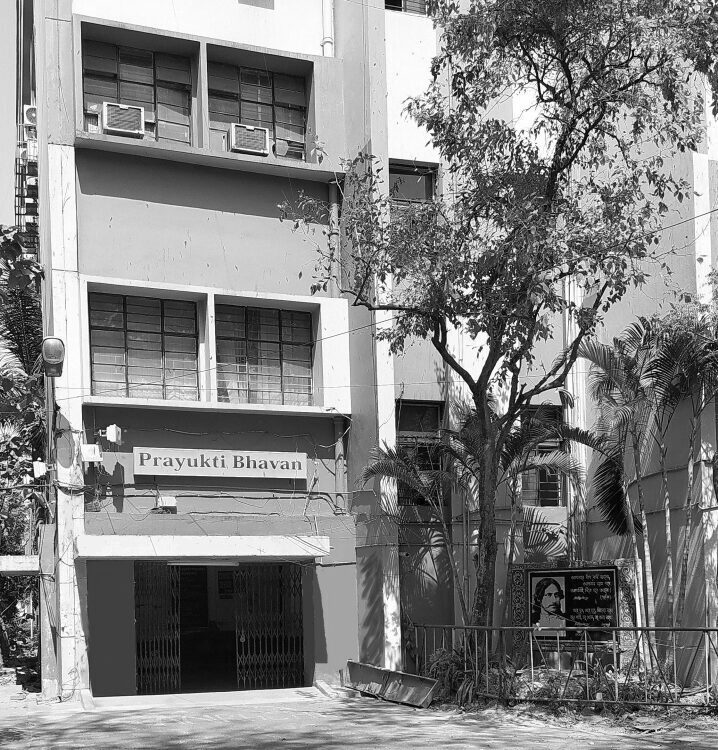
\includegraphics[width=0.3\linewidth]{images/prayukti.jpg}}
  \raisebox{-0.55\height}{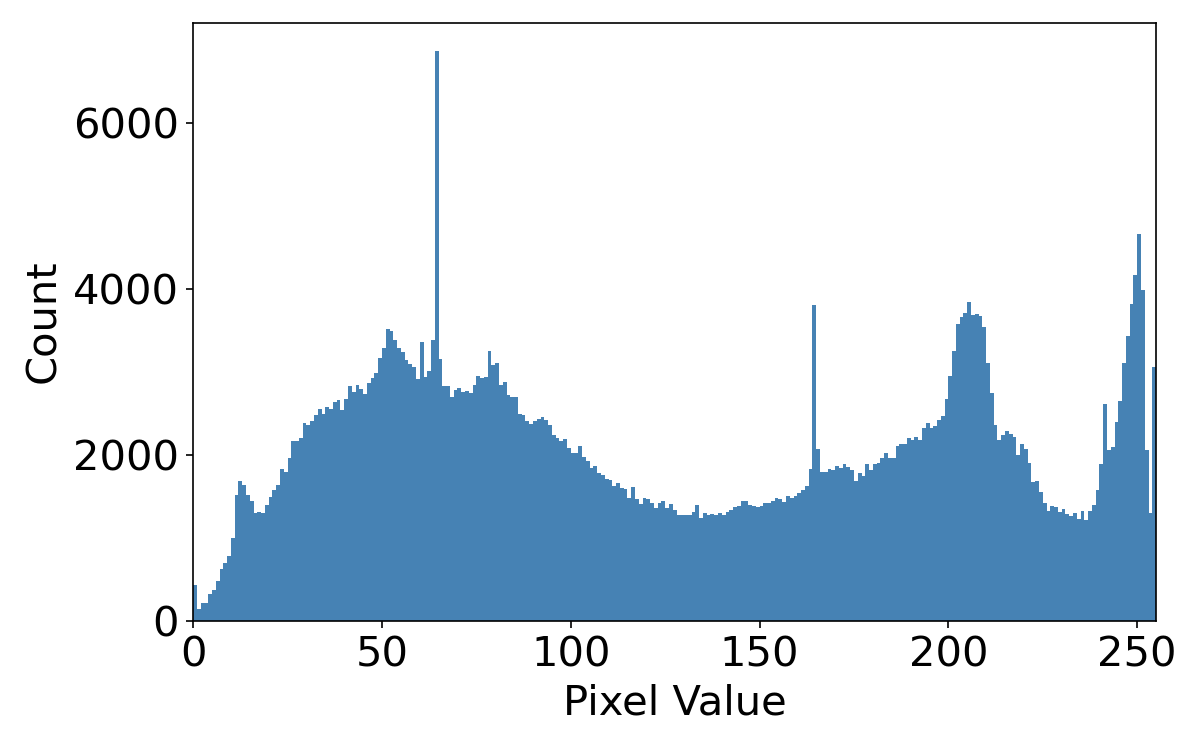
\includegraphics[width=0.6\linewidth]{images/prayukti_histogram.png}}
  \caption{Example image and its histogram}
\end{figure}

\subsection*{Contrast Stretching}

Contrast stretching (normalization) linearly expands an image’s
dynamic range, making low-contrast images more vivid. It’s the
simplest boost, though it can exaggerate noise or outliers.

\begin{equation*}
  s_k = T(r_k)
  = \frac{r_k - r_{\min}}{r_{\max} - r_{\min}}
  \times (L - 1)
\end{equation*}

where: (i) $r_k\rightarrow$ input intensity, (ii) $s_k\rightarrow$
output intensity, (iii) $r_{\min},\,r_{\max}\rightarrow$ observed
minimum and maximum intensities in the image, (iv) $L\rightarrow$
number of possible intensity levels

\begin{algorithm}[ht!]
  \DontPrintSemicolon
  Find $r_{\min}$ and $r_{\max}$ in input image $I$ \;

  {
    Apply T to each pixel intensity $r_k$ in $I$ \;
    \nonl $s_k \leftarrow \bigl(r_k -
    r_{\min}\bigr)\,/\,\bigl(r_{\max}-r_{\min}\bigr)\times(L-1)$ \;
    \nonl where $L$ is the number of intensity levels \;
  }

  Return contrast-stretched image $I'$\;
  \caption{Contrast Stretching}
\end{algorithm}

\subsection*{Histogram Equalization}

Refers to \enquote{spreading out} (equalizing) the frequencies in an
image. Simple way to improve dark or washed out images.

\begin{equation*}
  s_k = T(r_k) = \sum_{j=1}^{k} p_r(r_j) = \sum_{j=1}^{k} \frac{n_j}{n}
\end{equation*}

where: (i) $r_k \rightarrow$ input intensity, (ii) $s_k \rightarrow$
processed intensity, (iii) $k \rightarrow$ intensity range (e.g. 0 -
1), (iv) $n_j \rightarrow$ frequency of intensity $j$, (v) $n
\rightarrow$ total number of pixels (v) $L\rightarrow$ number of
possible intensity levels

\begin{algorithm}[ht!]
  \DontPrintSemicolon
  Compute histogram of input image $I$ \;
  Compute CDF from histogram \;
  Normalize CDF by dividing by $n$ \;

  {
    Apply $T$ to each pixel intensity $r_k$ in $I$\\
    \nonl $s_k = \text{CDF}[r_k] \times (L - 1)$ \\
    \nonl where $L$ is the number of intensity levels \;
  }

  Return enhanced image $I'$\;
  \caption{Histogram Equalization}
\end{algorithm}

\subsection*{Point Processing}

Simplest spatial domain operation, neighborhood is the pixel itself.

\subsubsection*{Negative Images}

Simply inverts pixel values; useful for enhancing dark regions.
\begin{equation*}
  s = (L - 1) - r
\end{equation*}

\subsubsection*{Thresholding}

Segments an image by \textbf{converting it to binary} based on a
threshold value (say $\theta_0$); useful for isolating objects from
the background.

\begin{equation*}
  s =
  \begin{cases}
    0 & \text{if } r < \theta_0 \\
    L - 1 & \text{if } r \geq \theta_0
  \end{cases}
\end{equation*}

\subsubsection*{Gray Level Transforms}

\begin{figure}[H]
  \centering
  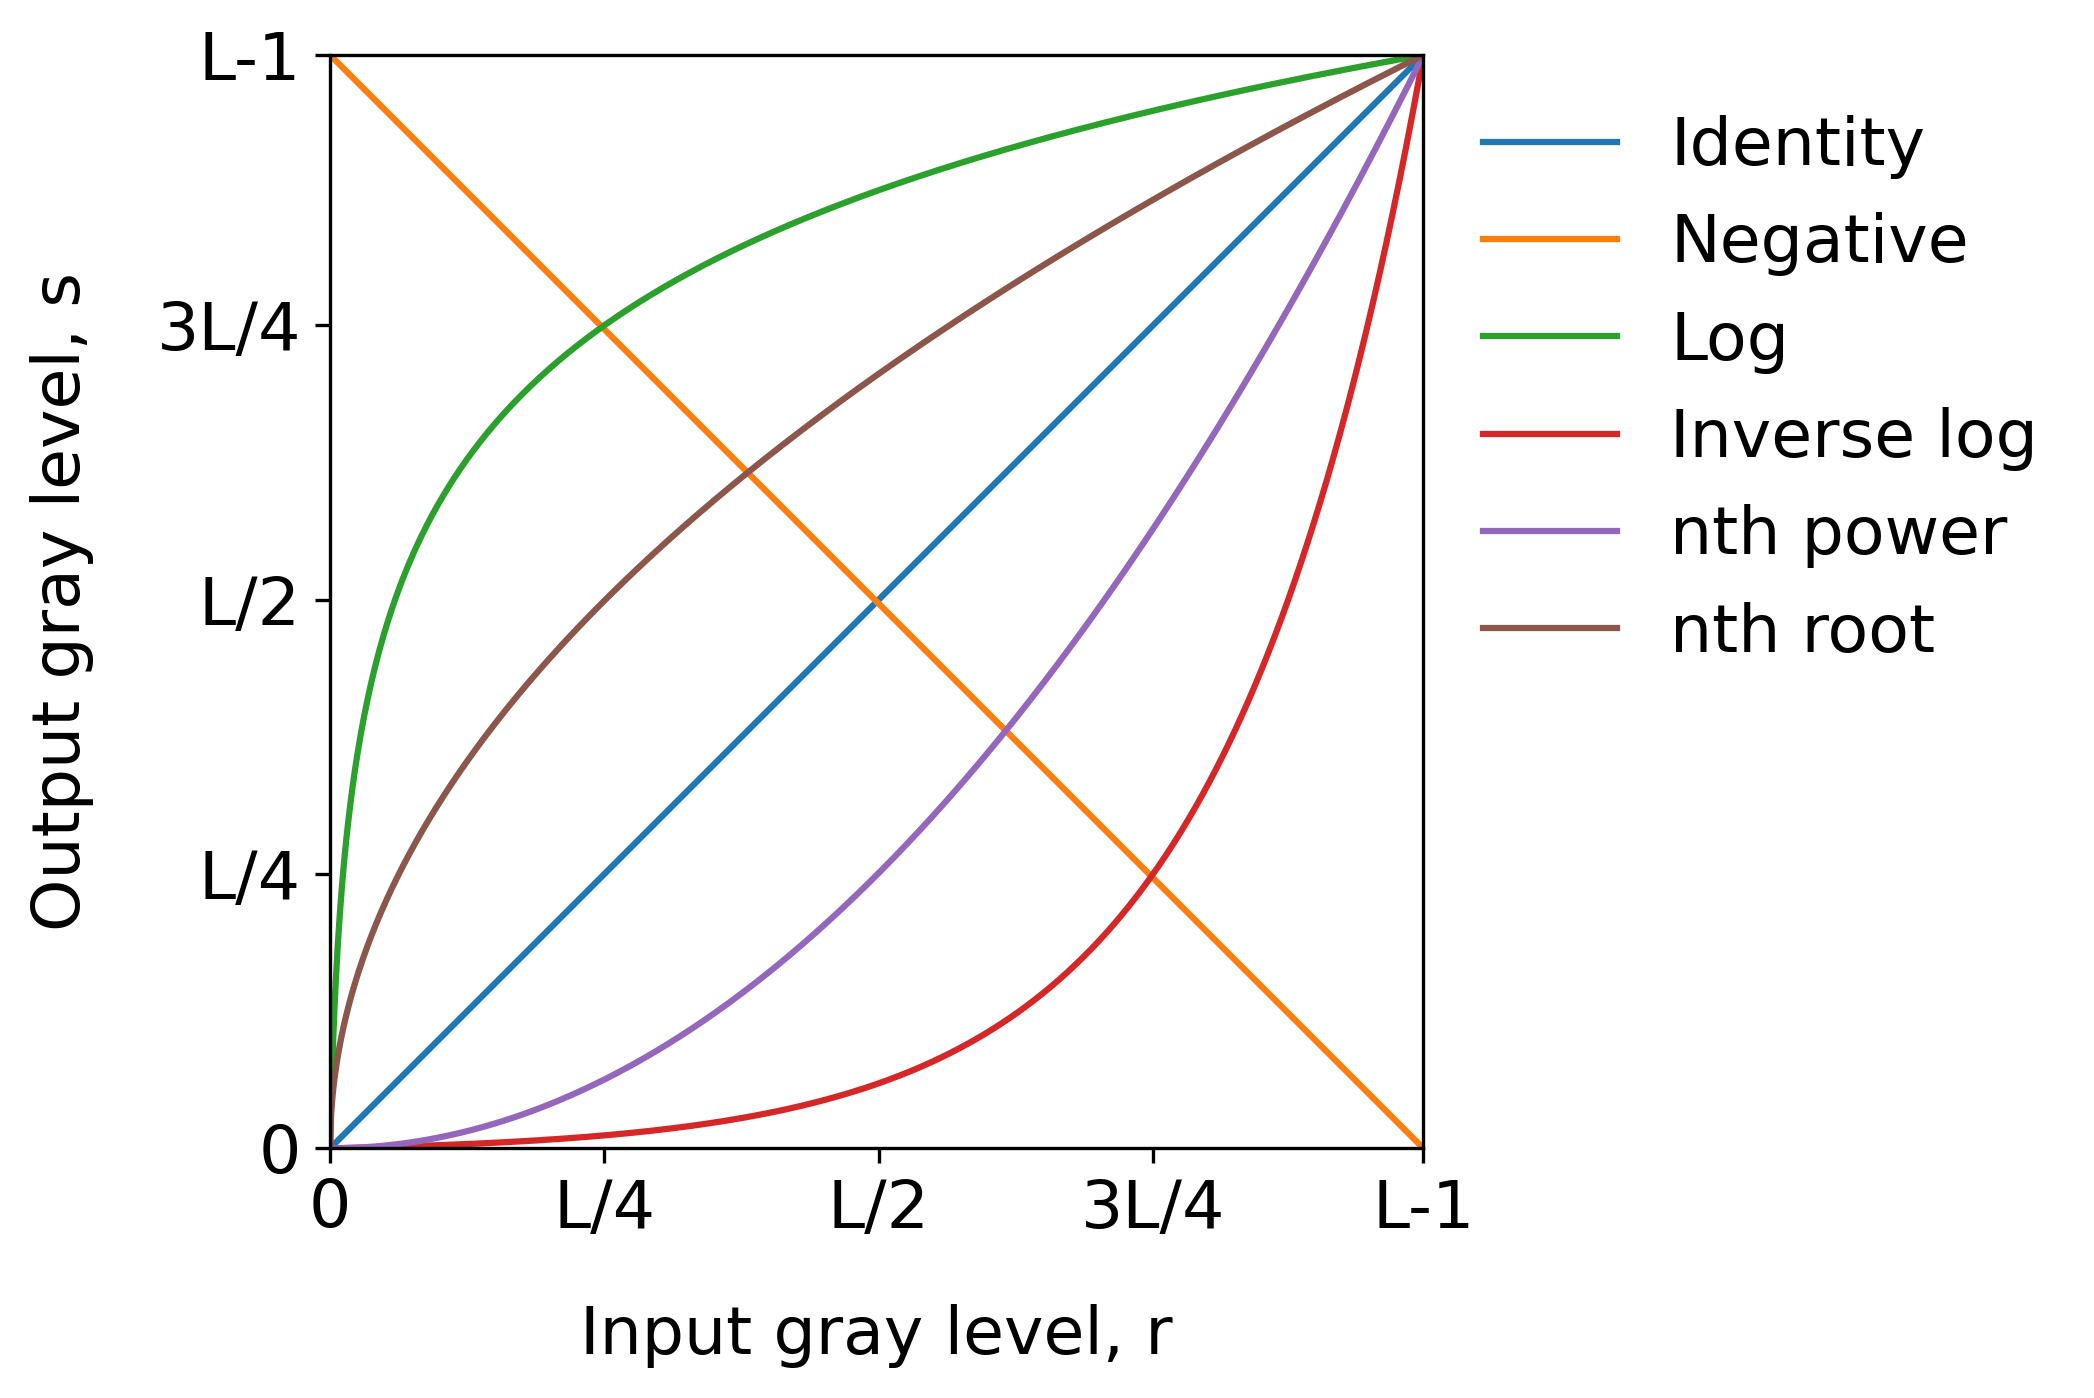
\includegraphics[width=\linewidth]{images/gray_level_transforms.png}
  \caption{Gray level transforms}
\end{figure}

\begin{itemize}
  \item \textbf{Log Transform:} Maps a narrow range of low input grey
    level values into a wider range of output values.
    \begin{itemize}
      \item $s = c \times \log(1 + r)$, where $c$ is a constant
      \item Useful when the input grey level values may have an
        extremely large range of values
      \item Use case 1: \textbf{log transform on Fourier transform}.
        More details are revealed.
      \item Use case 2: \textbf{gamma correction in displays}. Some
        displays do not respond linearly to different intensities;
        can be corrected using log transform
    \end{itemize}

  \item \textbf{Power Law Transform:} Maps a narrow range of dark
    input grey level values into a wider range of output values.
    \begin{itemize}
      \item $s = c \times r^{\gamma}$, where $\gamma$ is a constant
      \item Different $\gamma$ values highlight different details
      \item Useful for enhancing images with high dynamic range
    \end{itemize}

  \item \textbf{Piecewise Linear Transform:} Combines multiple
    arbitrary user-defined linear segments to create a more complex mapping.
    \begin{itemize}
      \item Useful for enhancing specific ranges of pixel values
      \item Can be used to adjust contrast in specific regions of an image
    \end{itemize}

    \begin{minipage}{\linewidth}
      \vspace{-0.5cm}
      \begin{figure}[H]
        \centering
        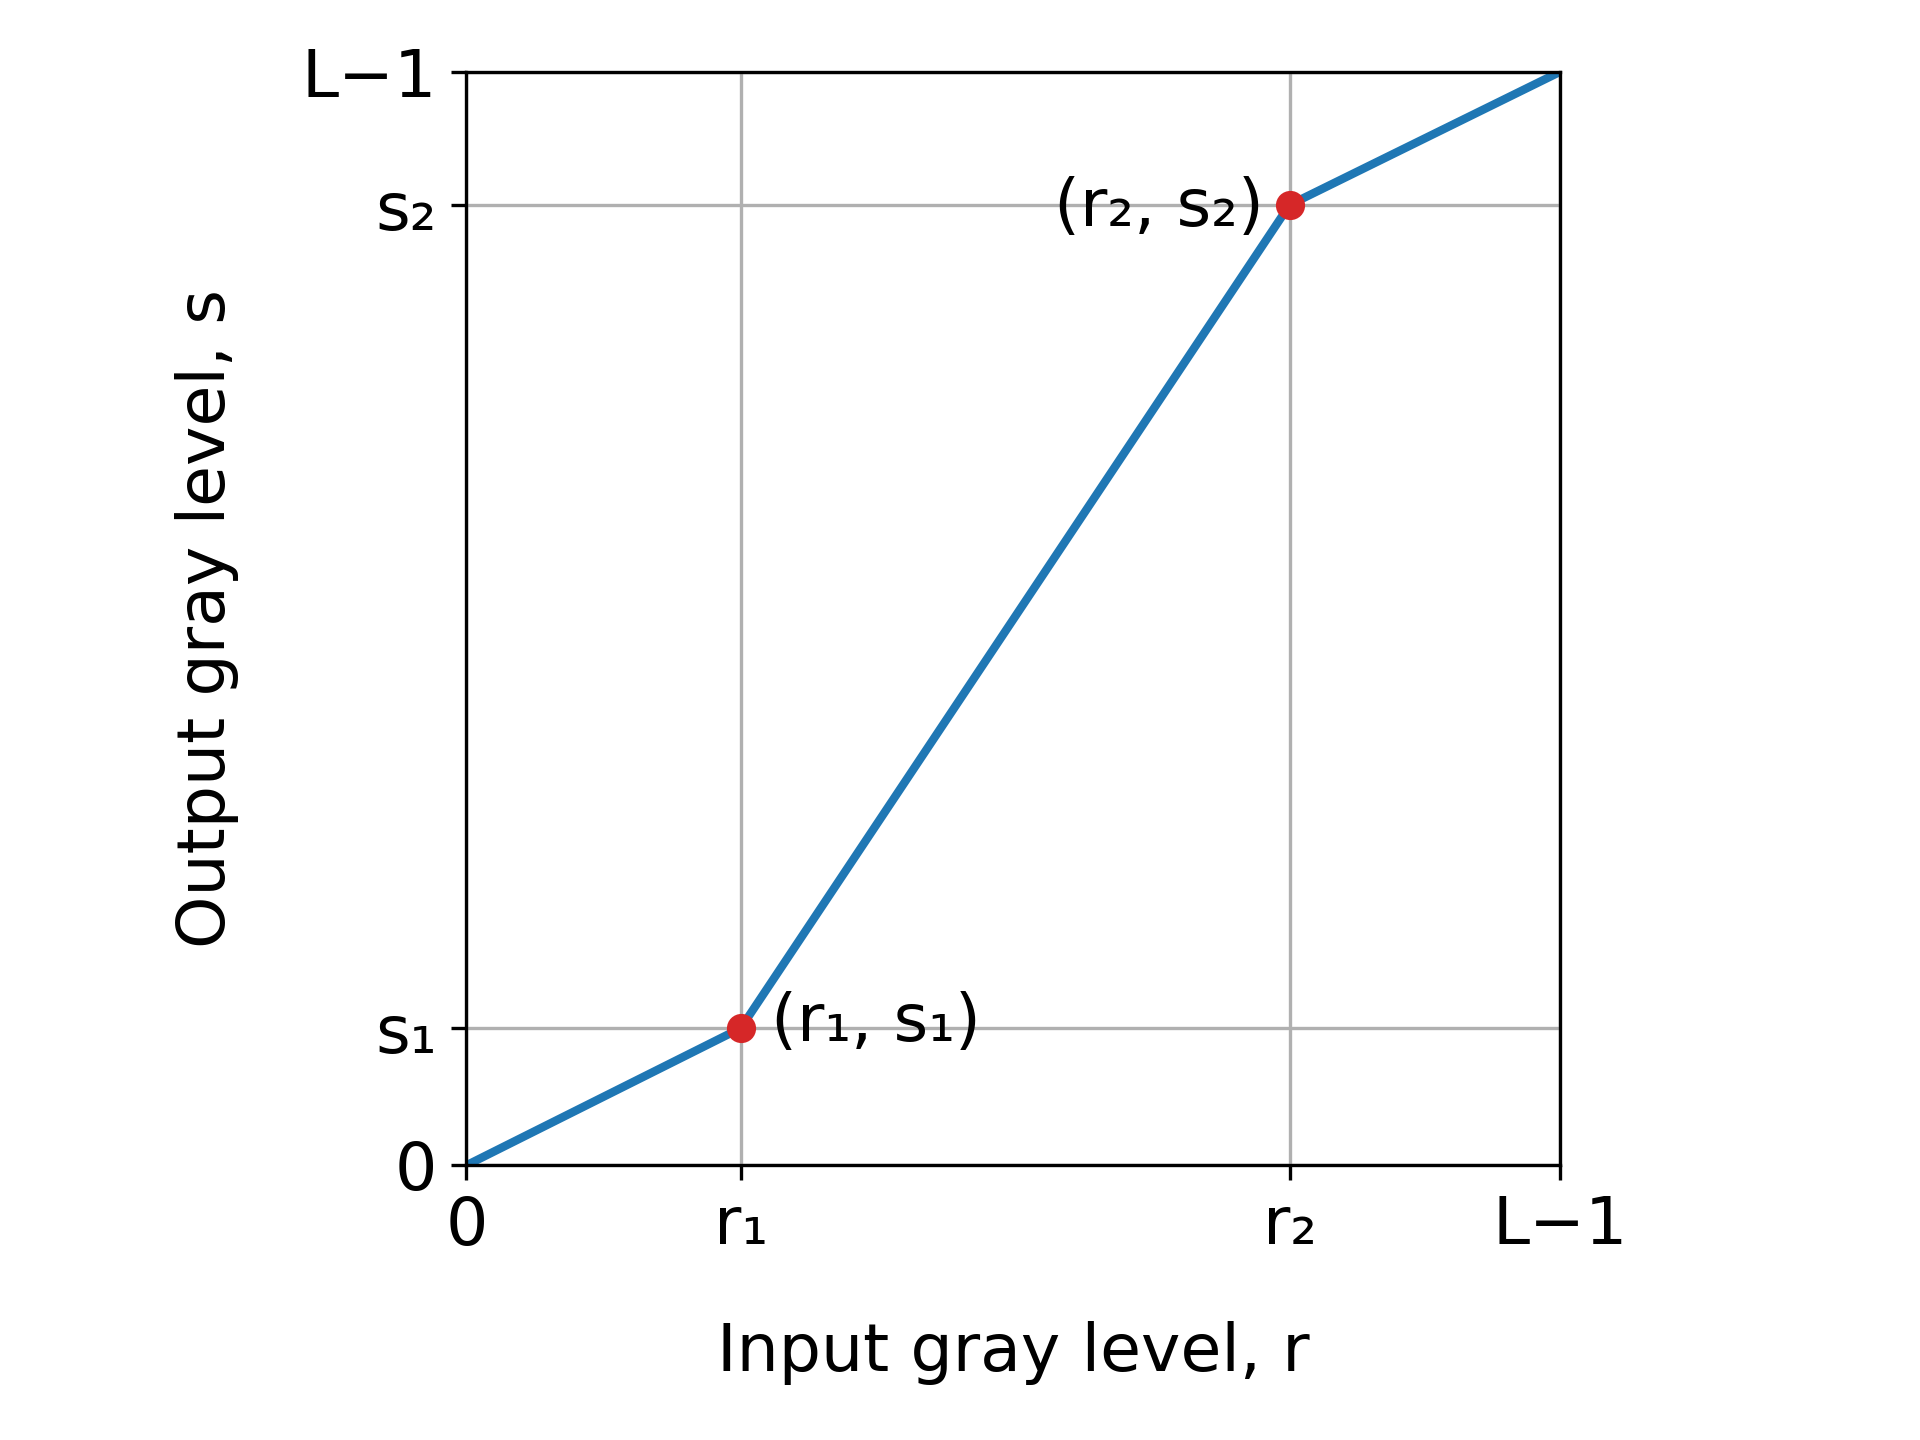
\includegraphics[width=\linewidth]{images/piecewise_transform.png}
        \vspace{-0.5cm}
        \caption{Piecewise linear transform}
      \end{figure}
    \end{minipage}

  \item \textbf{Gray Level Slicing:} Similar to thresholding, but
    allows for a range of pixel values to be highlighted.
    \begin{itemize}
      \item Other levels can be suppressed or maintained
      \item Useful for enhancing specific features in an image
    \end{itemize}

    \begin{minipage}{\linewidth}
      \begin{figure}[H]
        \centering
        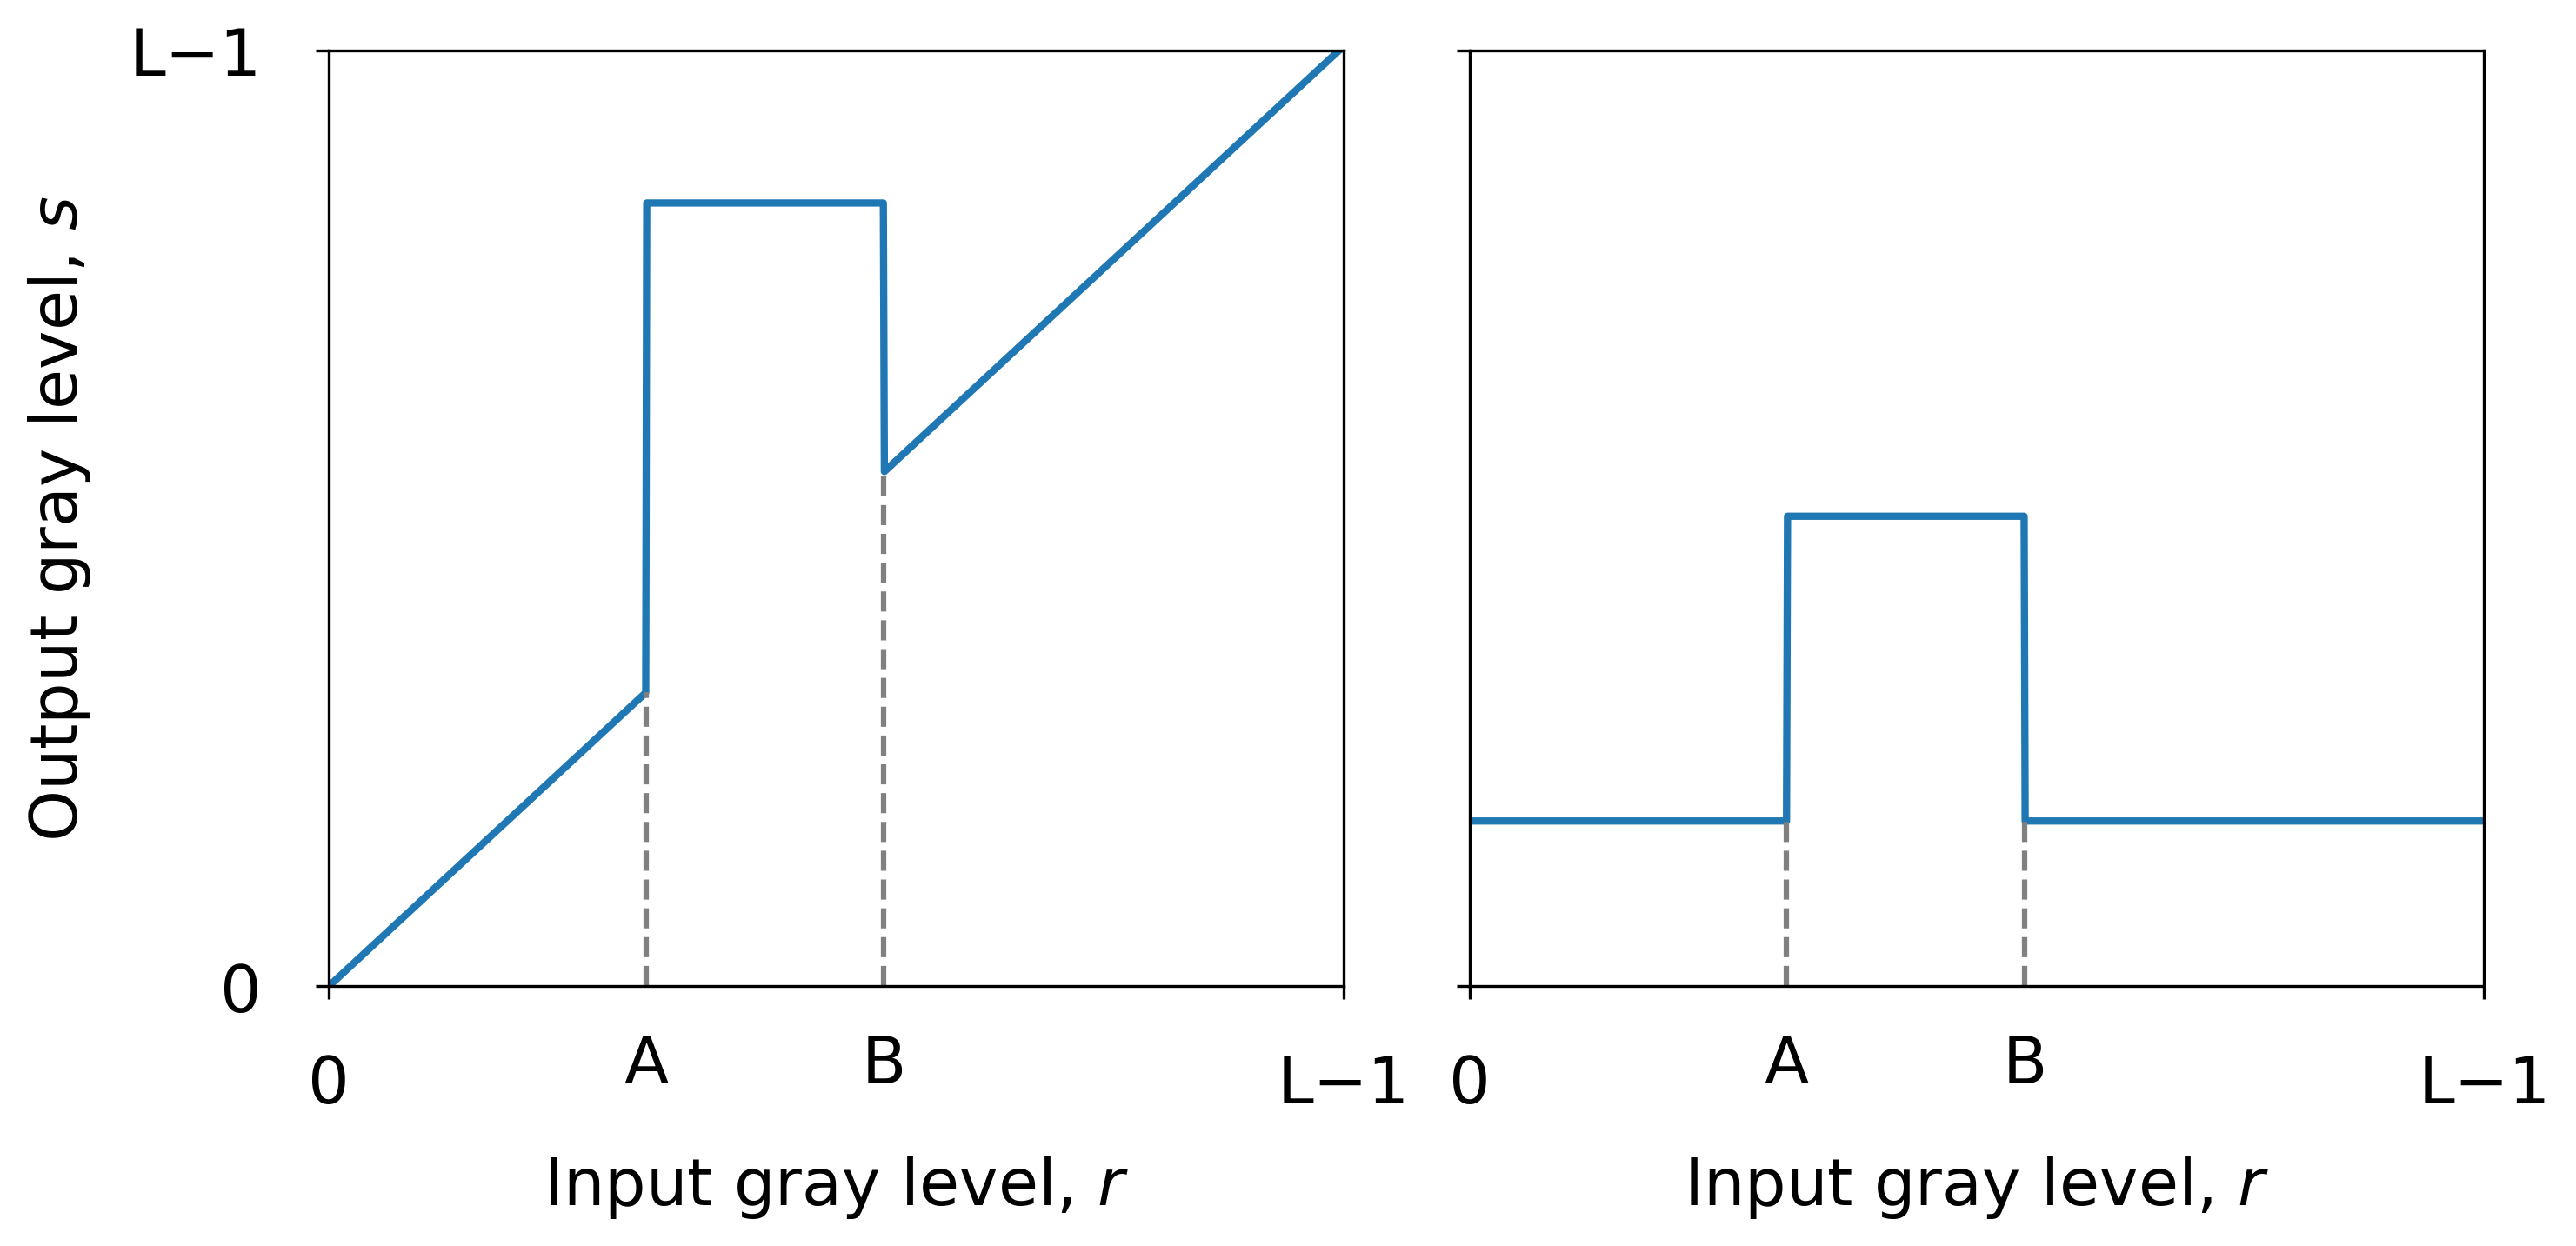
\includegraphics[width=\linewidth]{images/gray_level_slicing.png}
        \caption{Gray level slicing with (i) background retained (ii)
        background supressed}
      \end{figure}
    \end{minipage}

  \item \textbf{Bit-Plane Slicing:} By isolating particular bits of
    the pixel values in an image, we can highligh interesting aspects
    of that image.
    \begin{itemize}
      \item Higher order bits contain most of the significant information
      \item Lower order bits contain subtle details
      \item \enquote{Bit planes} are arranged in a stack; MSB at the
        top, LSB at the bottom.
    \end{itemize}

    \begin{minipage}{\linewidth}
      \begin{figure}[H]
        \centering
        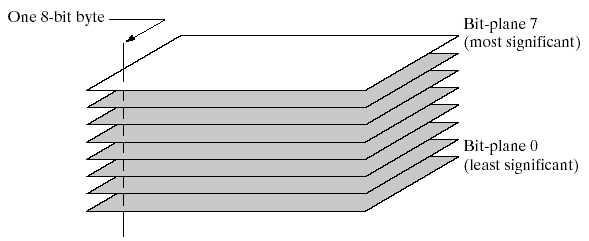
\includegraphics[width=\linewidth]{images/bit_plane_slicing.png}
        \caption{Bit-plane slicing of an 8-bit image}
      \end{figure}
      \vspace{-0.5cm}
    \end{minipage}

\end{itemize}

\subsection*{Neighborhood Operations}

Operations on a \textbf{rectangular region} around a pixel. Any size
rectangle and any shape filter are possible.

\subsubsection*{Simple Neighborhood Operations}

For any pixel $p$ in an image at the center of a neighborhood:

\begin{itemize}
  \item \textbf{Min:} Sets $p$ to minimum value in the neighborhood.
    \begin{itemize}
        \vspace{-0.2cm}
      \item Removes small bright spots (\textbf{salt noise})
      \item Makes \textbf{dark regions darker}
    \end{itemize}
  \item \textbf{Max:} Sets $p$ to maximum value in the neighborhood.
    \begin{itemize}
        \vspace{-0.2cm}
      \item Removes small dark spots (\textbf{pepper noise})
      \item Makes \textbf{bright regions brighter}
    \end{itemize}
  \item \textbf{Median:} Sets $p$ to median value in the neighborhood.
    \begin{itemize}
        \vspace{-0.2cm}
      \item Removes \textbf{salt and pepper noise}
    \end{itemize}
\end{itemize}

\subsubsection*{Spatial Differentiation}

Differentiation measures the \textit{rate of change} of a function.
In the context of image processing, the function is the pixel
intensity, and differentiation helps identify edges and transitions
in the image.

\begin{itemize}
  \item \textbf{First Derivative:} Measures the rate of change of
    pixel intensity.
    \begin{gather*}
      \frac{\partial f}{\partial x} = f(x + 1, y) - f(x, y)\\
      \frac{\partial f}{\partial y} = f(x, y + 1) - f(x, y)
    \end{gather*}
  \item \textbf{Second Derivative:} Measures the rate of change of
    the first derivative.
    \begin{gather*}
      \frac{\partial^2 f}{\partial x^2} = f(x + 1, y) + f(x - 1, y) - 2f(x, y)\\
      \frac{\partial^2 f}{\partial y^2} = f(x, y + 1) + f(x, y - 1) - 2f(x, y)
    \end{gather*}
  \item \textbf{The Laplacian:} Combines the second derivatives in
    both x and y directions.
    \begin{equation*}
      \nabla^2 f = \frac{\partial^2 f}{\partial x^2} +
      \frac{\partial^2 f}{\partial y^2}
    \end{equation*}
    In practice, the Laplacian is applied using a \textbf{filter}.
\end{itemize}

\begin{tblr}{
    colspec={@{}l X[l] | X[l]},
    row{1} = {c, font=\bfseries},
  }
  \cline{2-3}
  & \textbf{First Derivative} & \textbf{Second Derivative} \\
  \cline{2-3}
  \textbullet & Generally produces thicker edges
  & Stronger response to fine detail (e.g.\ thin lines) \\[6pt]
  \textbullet & Stronger response to grey level step
  & Double response to step changes in grey level \\[6pt]
\end{tblr}

\subsubsection*{Correlation vs Convolution}

Most spatial filtering operations are technically
\textbf{correlation}, and the filter is referred to as a
\textbf{correlation kernel} or \textbf{mask}. \textbf{Convolution} is
a similar operation, with a subtle difference:

\begin{figure}[H]
  \centering
  \begin{tikzpicture}[%
      imgcell/.style={draw=black, fill=white, minimum size=1cm, anchor=center},
      filtercell/.style={draw=MaterialBlue900, fill=MaterialBlue50,
      minimum size=1cm, anchor=center}
    ]

    % Original image grid
    \node[imgcell] (i11) at (0,2) {$r_1$};
    \node[imgcell] (i12) at (1,2) {$r_2$};
    \node[imgcell] (i13) at (2,2) {$r_3$};
    \node[imgcell] (i21) at (0,1) {$r_4$};
    \node[imgcell, fill=MaterialGrey200] (i22) at (1,1) {$r_5$};
    \node[imgcell] (i23) at (2,1) {$r_6$};
    \node[imgcell] (i31) at (0,0) {$r_7$};
    \node[imgcell] (i32) at (1,0) {$r_8$};
    \node[imgcell] (i33) at (2,0) {$r_9$};

    % Convolution symbol
    \node at (3,1) {\large $\ast$};

    % Filter grid
    \node[filtercell] (f11) at (4,2) {$k_1$};
    \node[filtercell] (f12) at (5,2) {$k_2$};
    \node[filtercell] (f13) at (6,2) {$k_3$};
    \node[filtercell] (f21) at (4,1) {$k_4$};
    \node[filtercell] (f22) at (5,1) {$k_5$};
    \node[filtercell] (f23) at (6,1) {$k_6$};
    \node[filtercell] (f31) at (4,0) {$k_7$};
    \node[filtercell] (f32) at (5,0) {$k_8$};
    \node[filtercell] (f33) at (6,0) {$k_9$};

  \end{tikzpicture}
  \caption{An image (left) being operated on by a filter (right). The
    result depends
  on whether the operation is correlation or convolution.}
\end{figure}
\vspace{-0.5cm}
\begin{itemize}
  \item \textbf{Correlation:} The filter is applied directly to the
    image, without flipping it.
    \vspace{-0.2cm}
    \begin{equation*}
      s = r_1 k_1 + r_2 k_2 + r_3 k_3 + r_4 k_4 + r_5 k_5 + r_6 k_6 +
      r_7 k_7 + r_8 k_8 + r_9 k_9\\[-0.3cm]
    \end{equation*}
  \item \textbf{Convolution:} The filter is flipped both horizontally
    and vertically before being applied to the image.
    \vspace{-0.2cm}
    \begin{equation*}
      s = r_1 k_9 + r_2 k_8 + r_3 k_7 + r_4 k_6 + r_5 k_5 + r_6 k_4 +
      r_7 k_3 + r_8 k_2 + r_9 k_1\\[-0.3cm]
    \end{equation*}
\end{itemize}

\subsubsection*{Handling Boundary Effects}

Edge pixels don't have a full neighborhood. A filter applied on a
pixel on or near the image boundaries \textbf{may exceed the image
boundaries}, leading to undefined behavior. There are strategies to
handle this:

\begin{minipage}{\linewidth}
  \begin{figure}[H]
    \centering
    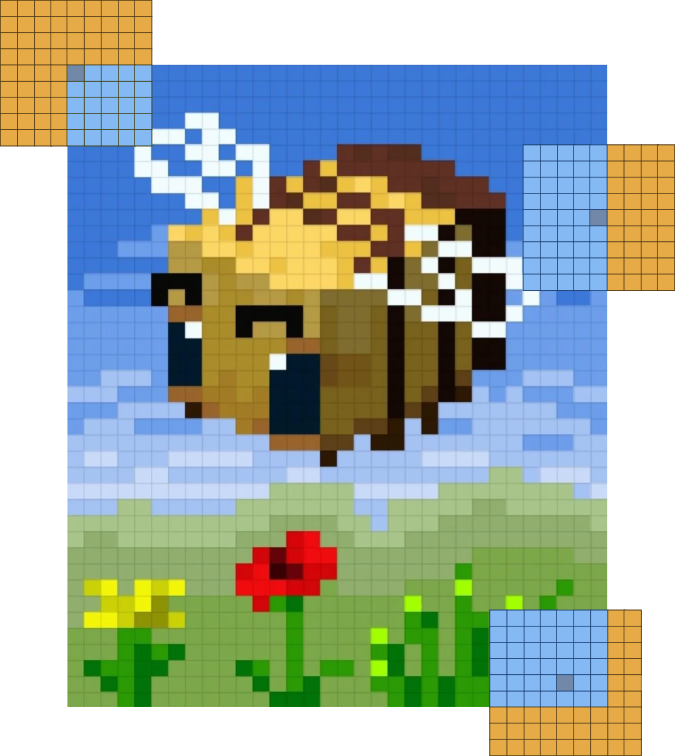
\includegraphics[width=0.6\linewidth]{images/edges.png}
    \caption{A filter may exceed the image boundaries}
  \end{figure}
\end{minipage}

\begin{itemize}
  \item \textbf{Valid (Crop)}: Only compute outputs where the kernel
    lies entirely inside; reduces output size.
  \item \textbf{Partial (Truncate)}: Ignore kernel weights falling
    outside and renormalize the remainder; minor overhead.
  \item \textbf{Constant Pad}: Add a border of fixed-value pixels
    (e.g.\ zero or white) to restore full output dimensions.
  \item \textbf{Replicate}: Extend the nearest edge pixel values
    outward; simple and fast, with minimal artifacts.
  \item \textbf{Reflect}: Mirror the image at its borders; preserves
    continuity but may introduce mirrored features.
\end{itemize}

\subsubsection*{Linear Spatial Filters}

\begin{equation*}
  g(x, y) = \sum_{s=-a}^{a} \sum_{t=-b}^{b} w(s, t) f(x + s, y + t)
\end{equation*}

\begin{itemize}
  \item \textbf{Identity Filter:} Leaves the image unchanged. Simply
    assigns a weight \enquote{0} to all the neighbors around the central pixel.

    \begin{minipage}{\linewidth}
      \vspace{-0.3cm}
      \begin{figure}[H]
        \centering
        \begin{tikzpicture}[%
            filtercell/.style={draw=MaterialBlue900, fill=MaterialBlue50,
            minimum size=1cm, anchor=center}
          ]
          \node[filtercell] (f11) at (0,2) {$0$};
          \node[filtercell] (f12) at (1,2) {$0$};
          \node[filtercell] (f13) at (2,2) {$0$};
          \node[filtercell] (f21) at (0,1) {$0$};
          \node[filtercell] (f22) at (1,1) {$1$};
          \node[filtercell] (f23) at (2,1) {$0$};
          \node[filtercell] (f31) at (0,0) {$0$};
          \node[filtercell] (f32) at (1,0) {$0$};
          \node[filtercell] (f33) at (2,0) {$0$};

        \end{tikzpicture}
        \caption{Identity filter}
      \end{figure}
    \end{minipage}
  \item \textbf{Smoothing Filters:} Smooths an image by averaging
    pixel values in the neighborhood.
    \begin{itemize}
      \item \textbf{Mean filter} or \textbf{simple
        averaging filter}: simplest form; $k \times k$ matrix, each
        element is $1/k^2$.

        \begin{minipage}{\linewidth}
          \vspace{-0.3cm}
          \begin{figure}[H]
            \centering
            \begin{tikzpicture}[%
                filtercell/.style={draw=MaterialBlue900, fill=MaterialBlue50,
                minimum size=1cm, anchor=center}
              ]
              \node[filtercell] (f11) at (0,2) {$1/9$};
              \node[filtercell] (f12) at (1,2) {$1/9$};
              \node[filtercell] (f13) at (2,2) {$1/9$};
              \node[filtercell] (f21) at (0,1) {$1/9$};
              \node[filtercell] (f22) at (1,1) {$1/9$};
              \node[filtercell] (f23) at (2,1) {$1/9$};
              \node[filtercell] (f31) at (0,0) {$1/9$};
              \node[filtercell] (f32) at (1,0) {$1/9$};
              \node[filtercell] (f33) at (2,0) {$1/9$};

            \end{tikzpicture}
            \caption{Simple 3x3 averaging filter}
          \end{figure}
        \end{minipage}
      \item \textbf{Weighted averaging filter}: Sometimes different
        pixels in the neighborhood are weighted differently; the
        filter values always add up to 1.

        \begin{minipage}{\linewidth}
          \vspace{-0.3cm}
          \begin{figure}[H]
            \centering
            \begin{tikzpicture}[%
                filtercell/.style={draw=MaterialBlue900, fill=MaterialBlue50,
                minimum size=1cm, anchor=center}
              ]
              \node[filtercell] (f11) at (0,2) {$1/16$};
              \node[filtercell] (f12) at (1,2) {$2/16$};
              \node[filtercell] (f13) at (2,2) {$1/16$};
              \node[filtercell] (f21) at (0,1) {$2/16$};
              \node[filtercell] (f22) at (1,1) {$4/16$};
              \node[filtercell] (f23) at (2,1) {$2/16$};
              \node[filtercell] (f31) at (0,0) {$1/16$};
              \node[filtercell] (f32) at (1,0) {$2/16$};
              \node[filtercell] (f33) at (2,0) {$1/16$};

            \end{tikzpicture}
            \caption{Weighted 3x3 averaging filter}
          \end{figure}
        \end{minipage}

      \item \textbf{Useful for}: (i) removing noise from images (ii)
        highlighting gross details
    \end{itemize}
  \item \textbf{Sharpening Filters:} Enhances edges, removes blurring
    and fine details in an image.
    \begin{itemize}
      \item \textbf{Laplacian Filter:} Highlights regions of rapid
        intensity change (edges and other discontinuities).
        \begin{itemize}
          \item The Laplacian output is \textbf{not an enhanced
            image}; it is an image with those regions highlighted,
            where the pixel values change rapidly in the original
            image (edges etc.)
          \item In order to obtain the enhanced image, the Laplacian
            output is \textbf{subtracted} from the original image.
          \item This above operation can be summarized as a new
            filter: identity minus Laplacian.
        \end{itemize}

        \begin{minipage}{\linewidth}
          \vspace{-0.3cm}
          \begin{figure}[H]
            \centering
            \begin{tikzpicture}[%
                filtercell/.style={draw=MaterialBlue900, fill=MaterialBlue50,
                minimum size=1cm, anchor=center}
              ]
              \node[filtercell] (f111) at (0,2) {$0$};
              \node[filtercell] (f112) at (1,2) {$1$};
              \node[filtercell] (f113) at (2,2) {$0$};
              \node[filtercell] (f121) at (0,1) {$1$};
              \node[filtercell] (f122) at (1,1) {$4$};
              \node[filtercell] (f123) at (2,1) {$1$};
              \node[filtercell] (f131) at (0,0) {$0$};
              \node[filtercell] (f132) at (1,0) {$1$};
              \node[filtercell] (f133) at (2,0) {$0$};

              \node[filtercell] (f211) at (4,2) {$0$};
              \node[filtercell] (f212) at (5,2) {$-1$};
              \node[filtercell] (f213) at (6,2) {$0$};
              \node[filtercell] (f221) at (4,1) {$-1$};
              \node[filtercell] (f222) at (5,1) {$5$};
              \node[filtercell] (f223) at (6,1) {$-1$};
              \node[filtercell] (f231) at (4,0) {$0$};
              \node[filtercell] (f232) at (5,0) {$-1$};
              \node[filtercell] (f233) at (6,0) {$0$};
            \end{tikzpicture}
            \caption{Laplacian filter (left), Identity minus
            Laplacian filter (right)}
          \end{figure}
        \end{minipage}

      \item \textbf{Unsharp Mask and High-Boost Filtering:} These are
        filters that enhance edges by subtracting a blurred version
        of the image ($\bar{f}(x, y)$) from the original image ($f(x, y)$)
        \begin{gather*}
          f_\textnormal{s}(x, y) = f(x, y) - \bar{f}(x, y)\\
          f_\textnormal{hb}(x, y) = Af(x, y) - \bar{f}(x, y)
        \end{gather*}
        \begin{itemize}
          \item High-boost filtering ($f_\textnormal{hb}$) takes a
            strength parameter $A$. Unsharp mask ($f_\textnormal{s}$)
            is a special case of high-boost filtering with $A = 1$.
        \end{itemize}
    \end{itemize}
    \begin{minipage}{\linewidth}
      \vspace{-0.3cm}
      \begin{figure}[H]
        \centering
        \begin{tikzpicture}[%
            filtercell/.style={draw=MaterialBlue900, fill=MaterialBlue50,
            minimum size=1cm, anchor=center}
          ]
          \node[filtercell] (f111) at (0,2) {$0$};
          \node[filtercell] (f112) at (1,2) {$-1$};
          \node[filtercell] (f113) at (2,2) {$0$};
          \node[filtercell] (f121) at (0,1) {$-1$};
          \node[filtercell] (f122) at (1,1) {\small \hspace{-0.5em} $A + 4$};
          \node[filtercell] (f123) at (2,1) {$-1$};
          \node[filtercell] (f131) at (0,0) {$0$};
          \node[filtercell] (f132) at (1,0) {$-1$};
          \node[filtercell] (f133) at (2,0) {$0$};

          \node[filtercell] (f211) at (4,2) {$-1$};
          \node[filtercell] (f212) at (5,2) {$-1$};
          \node[filtercell] (f213) at (6,2) {$-1$};
          \node[filtercell] (f221) at (4,1) {$-1$};
          \node[filtercell] (f222) at (5,1) {\small \hspace{-0.5em} $A + 8$};
          \node[filtercell] (f223) at (6,1) {$-1$};
          \node[filtercell] (f231) at (4,0) {$-1$};
          \node[filtercell] (f232) at (5,0) {$-1$};
          \node[filtercell] (f233) at (6,0) {$-1$};
        \end{tikzpicture}
        \caption{Two forms of unsharp mask}
      \end{figure}
    \end{minipage}

    For the specific case of a 3x3 filter, the unsharp mask perfectly
    matches the \enquote{identity minus Laplacian filter}!

  \item \textbf{Sobel Filters:} Based on 1st derivative filtering,
    these are typically used for edge detection.
    \begin{itemize}
      \item The Sobel filters are based on the calculation of
        gradients in the x and y directions. As such, there are two
        filters, one for $G_x$ and one for $G_y$.
      \item To filter an image, (i) both the filters are applied and
        (ii) the results are added together.
    \end{itemize}

    \begin{minipage}{\linewidth}
      \vspace{-0.3cm}
      \begin{figure}[H]
        \centering
        \begin{tikzpicture}[%
            filtercell/.style={draw=MaterialBlue900, fill=MaterialBlue50,
            minimum size=1cm, anchor=center}
          ]
          \node[filtercell] (f111) at (0,2) {$-1$};
          \node[filtercell] (f112) at (1,2) {$0$};
          \node[filtercell] (f113) at (2,2) {$1$};
          \node[filtercell] (f121) at (0,1) {$-2$};
          \node[filtercell] (f122) at (1,1) {$0$};
          \node[filtercell] (f123) at (2,1) {$2$};
          \node[filtercell] (f131) at (0,0) {$-1$};
          \node[filtercell] (f132) at (1,0) {$0$};
          \node[filtercell] (f133) at (2,0) {$1$};

          \node[filtercell] (f211) at (4,2) {$-1$};
          \node[filtercell] (f212) at (5,2) {$-2$};
          \node[filtercell] (f213) at (6,2) {$-1$};
          \node[filtercell] (f221) at (4,1) {$0$};
          \node[filtercell] (f222) at (5,1) {$0$};
          \node[filtercell] (f223) at (6,1) {$0$};
          \node[filtercell] (f231) at (4,0) {$1$};
          \node[filtercell] (f232) at (5,0) {$2$};
          \node[filtercell] (f233) at (6,0) {$1$};
        \end{tikzpicture}
        \caption{The Sobel filters for $G_x$/horizontal derivative
        (left) and $G_y$/vertical derivative (right)}
      \end{figure}
    \end{minipage}
\end{itemize}


\end{document}
